\chapter{Runtime Estimators: Training and Selection of Optimal Models for Inference}
\label{BuildEstimator.ch}

In this chapter, we discuss various loss functions and evaluation metrics used to assess model accuracy. We then explore both off-the-shelf and custom regression models for runtime estimation, detailing how metrics guide the selection of the best-performing model for a given application based on its characteristics and the availability of historical data (SD and FS samples).

\section{Loss Functions and Metrics}
As we develop estimation models, which primarily rely on regression techniques, they are typically trained using Mean Squared Error (MSE) as the default loss function. To evaluate and compare the performance of these models, metrics such as Mean Squared Error (MSE), Mean Absolute Error (MAE), or Root Mean Squared Error (RMSE) are commonly used.
Although resource (runtime) estimation models are regression-based, underestimations and overestimations have different consequences. Overestimations primarily lead to longer queue wait times, whereas underestimations can be more detrimental, often causing premature job termination and necessitating re-execution, leading to wasted computational resources. To address this imbalance, conventional loss functions need modifications to penalize underpredictions more heavily, ensuring better optimization during training. This type of adjustment is known as a biased loss function, and one well-known example is the Huber Loss function.

\begin{itemize}
    \item Mean Squared Error (MSE):The Mean Squared Error (MSE) measures the average squared difference between actual and predicted values:
    \begin{equation}
        MSE = \frac{1}{n} \sum_{i=1}^{n} (y_i - \hat{y}_i)^2 
    \end{equation}
     
    MSE has the advantage of penalizing larger errors more than smaller ones, making it useful for models that require higher sensitivity to outliers. However, the same characteristics make MSE is highly sensitive to outliers due to the squared term, which can disproportionately affect the loss
    \item Root Mean Squared Error (RMSE)
    The Root Mean Squared Error (RMSE) is the square root of the MSE, which brings the error back to the original unit of measurement:
    \begin{equation}
        RMSE = \sqrt{\frac{1}{n} \sum_{i=1}^{n} (y_i - \hat{y}_i)^2} 
    \end{equation} 
    RMSE maintains the same unit as the target variable, making it more interpretable and incomparable. 
    \item Mean Absolute Percentage Error (MAPE)
    The Mean Absolute Percentage Error (MAPE) measures error in percentage terms, making it scale-independent:
    \begin{equation}
        MAPE = \frac{100}{n} \sum_{i=1}^{n} \left| \frac{y_i - \hat{y}_i}{y_i} \right| 
    \end{equation} 
    MAPE expresses error as a percentage, making it easier to interpret across different datasets and is less sensitive to extreme values than MSE and RMSE; however, it cannot be used when actual values contain zero and tends to overweight small actual values, potentially skewing results
    \item Huber Loss: Huber Loss is a combination of MSE and MAE, designed to be robust against outliers by applying a quadratic loss for small errors and a linear loss for large errors:
    \begin{equation}
        L_{\delta}(a) =
        \begin{cases} 
        \frac{1}{2} a^2 & \text{for } |a| \leq \delta \\
        \delta (|a| - \frac{1}{2} \delta) & \text{for } |a| > \delta
        \end{cases}
    \end{equation}
    where: \( a = y - \hat{y} \) is the residual (difference between actual and predicted values). \( \delta \) is a threshold that determines the transition between MSE and MAE.
    Huber loss is less sensitive to outliers compared to MSE and RMSE, providing a balanced approach between squared and absolute error penalties. However, it requires tuning of the threshold parameter \( \delta \), which can be challenging, and is more complex to implement than MSE and RMSE.
    \item Under-Prediction Percentage in Resource Provisioning
    Under-prediction percentage measures the frequency at which a resource estimator predicts fewer resources than actually required, potentially leading to job failures due to insufficient allocation. It is defined as:

    \begin{equation}
    \text{Under-Prediction Percentage} = \frac{\sum ( \hat{y}_i < y_i )}{N} \times 100
    \end{equation}
    
    where \( \hat{y}_i \) is the predicted resource requirement for job \( i \), \( y_i \) is the actual resource usage, and \( N \) is the total number of jobs.
    
    Under-prediction percentage plays a crucial role in resource provisioning by ensuring conservative estimation and minimizing job failures caused by insufficient resource allocation. A lower under-prediction percentage helps optimize scheduling efficiency by refining estimations over time, thereby improving overall workload performance. Accurate prediction prevents job resubmissions and unnecessary system crashes, leading to better system reliability. Furthermore, minimizing under-prediction enhances adaptive learning in machine learning-based resource estimation models, ensuring that workloads receive adequate computing resources while balancing efficiency and cost.
    \item Asymmetric Custom Loss for Runtime Prediction: Developing a specialized loss function \cite{ehrig2020customizable} that optimizes the model to reduce under-predictions while minimizing the percentage error in overestimation.
    \begin{equation}
    L_H(x) =
    \begin{cases} 
        -\gamma_L(2x + \gamma_L), & \text{for } -\infty < x < -\gamma_L \\
        x^2, & \text{for } -\gamma_L \leq x < 0 \\
        x^2, & \text{for } 0 \leq x < \gamma_R \\
        \gamma_R(2x - \gamma_R), & \text{for } \gamma_R \leq x < \infty
    \end{cases}
    \label{Form:Custom_Assyn_Loss}
    \end{equation}
    where \( x = y_i - \hat{y}_i\), \( \gamma_L \) and \( \gamma_R \) are tunable constants to reduce the no. of underpredictions and minimize the overestimation error.

\end{itemize} 

Figure~\ref{fig:huber_loss} visualizes different loss functions, highlighting the impact of asymmetric penalties on overestimation and underestimation. The left-plot compares multiple Huber loss functions under various \(\gamma\) configurations, while the right-plot illustrates variations of the asymmetric Huber loss function for different asymmetry parameter values (\(\gamma_L\) and \(\gamma_R\)).

To fine-tune models for reducing underpredictions (reducing reruns) and minimizing overestimation errors (avoiding unnecessary wait times), optimizing the hyperparameters \(\gamma_L\) and \(\gamma_R\) is essential. From the right plot, the ideal loss function follows the "red-dashed line," which corresponds to \(\gamma_L = 0.1\) and \(\gamma_R = 0.9\).

\begin{figure}[h]
    \centering
    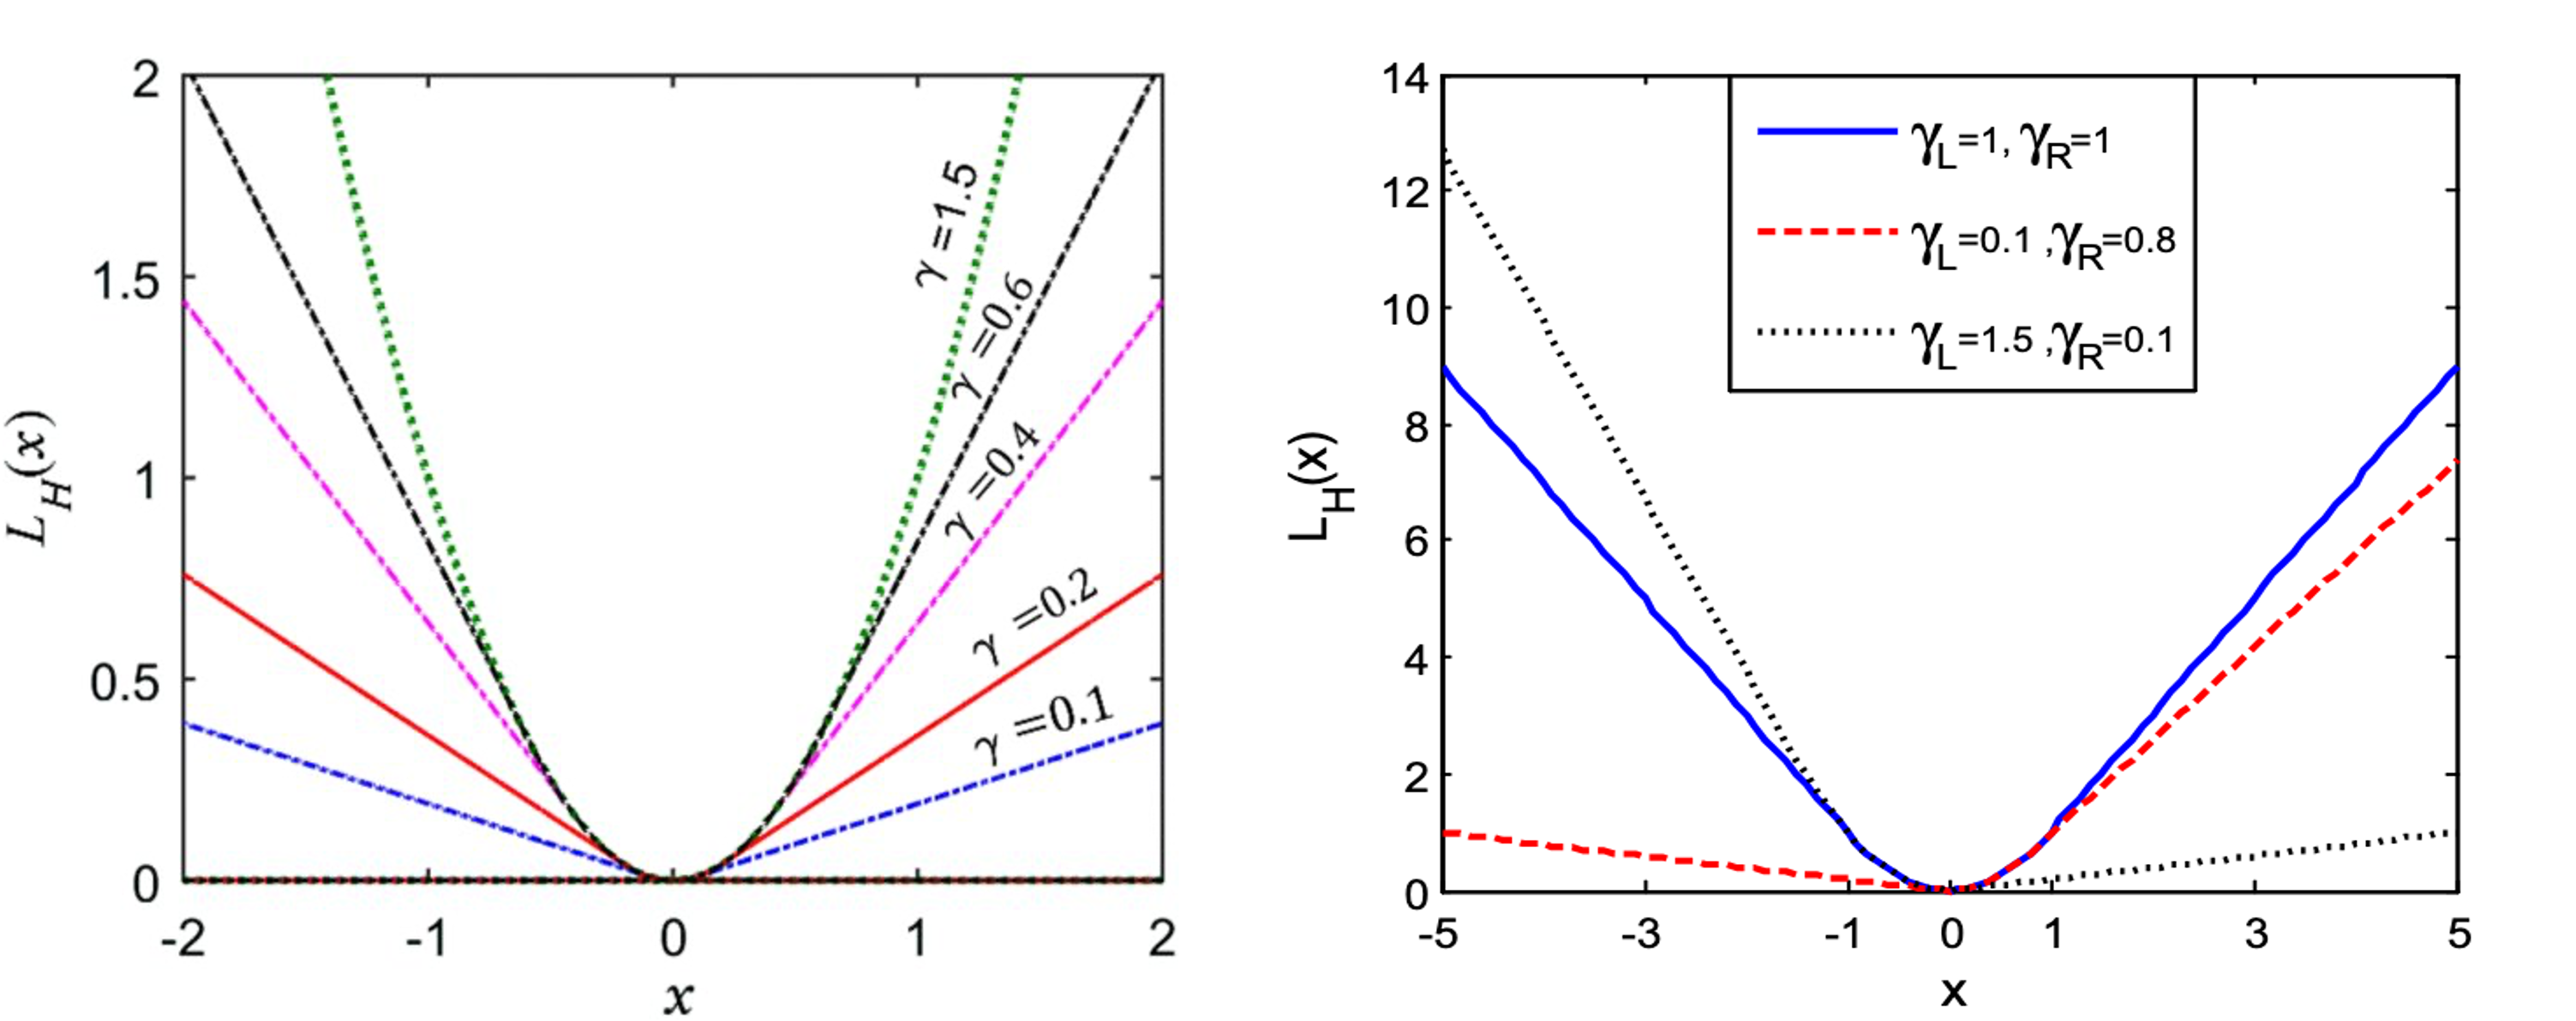
\includegraphics[width=0.95\textwidth]{Images/Loss.png}
    \caption{Comparison of different Huber-like loss functions for asymmetric error handling. The left plot illustrates the effect of different values of \(\gamma\) on the shape of the loss function, while the right plot presents multiple parameter settings for asymmetric loss variations, controlling how errors are penalized differently for underestimation and overestimation with \(\gamma_L\) and \(\gamma_R\)}
    \label{fig:huber_loss}
\end{figure}


\section{Candidate Regression Models}

Given the diverse characteristics of the training data, as shown in Figure~\ref{fig:features_overview} for each application, a single-model approach is not effective for all cases. For instance, Decision Tree regression models perform best when the training and test sets share the same distribution—both from scaled-down data or full-scale data (see Table~\ref{Data_Model}). However, a neural network-based or Linear Regression-based approach scales more effectively when training on scaled-down data and inferring on full-scale.



\subsection{Regression Models and Training Data Characteristics}

\subsubsection{Decision Tree Regressor}
\textbf{Description:} A non-parametric model that splits the data into decision nodes based on feature thresholds. It recursively partitions the dataset into smaller subsets, forming a tree structure.

\textbf{Ideal Training Data Characteristics:}
\begin{itemize}
    \item Works well with non-linear relationships.
    \item Handles both categorical and numerical features.
    \item Performs well with moderate-sized datasets but is prone to overfitting on small datasets.
    \item Sensitive to noisy data and requires pruning or regularization to prevent overfitting.
\end{itemize}

\subsubsection{Multiple Linear Regression}
\textbf{Description:} Multiple Linear Regression (MLR) is an extension of simple linear regression that models the relationship between a dependent variable \( Y \) and multiple independent variables \( X_1, X_2, ..., X_n \). It assumes a linear relationship between the predictors and the response, expressed as:

\begin{equation}
    Y = \beta_0 + \beta_1 X_1 + \beta_2 X_2 + ... + \beta_n X_n + \epsilon
\end{equation}

Where:
\begin{itemize}
    \item \( \beta_0 \) is the intercept, \( \beta_1, \beta_2, ..., \beta_n \) are the regression coefficients, and \( \epsilon \) is the error term.
\end{itemize}

\textbf{Ideal Training Data Characteristics:}
\begin{itemize}
    \item \textbf{Linearity Assumption:} The relationship between independent variables and the dependent variable should be approximately linear.
    \item \textbf{No Multicollinearity:} Independent variables should not be highly correlated with each other. Variance Inflation Factor (VIF) analysis helps detect multicollinearity.
    \item \textbf{Sufficient Data Points:} Works best with a dataset where the number of observations is significantly greater than the number of independent variables to avoid overfitting.
\end{itemize}

\subsubsection{Lasso Regression (L1 Regularization)}
\textbf{Description:} A linear regression model with L1 regularization that shrinks some coefficients to zero, effectively performing feature selection.

\textbf{Ideal Training Data Characteristics:}
\begin{itemize}
    \item Works well when there are many correlated features, as it selects the most relevant ones.
    \item Suitable for high-dimensional datasets where feature reduction is needed.
    \item Requires features to be standardized or normalized for better performance.
    \item Works best when some features are irrelevant or redundant in predicting the output.
\end{itemize}

\subsubsection{Support Vector Regression (SVR)}
\textbf{Description:} A kernel-based regression model that finds a function within a margin of tolerance (epsilon) while minimizing prediction errors. Uses kernel functions (linear, RBF, polynomial) to capture complex relationships.

\textbf{Ideal Training Data Characteristics:}
\begin{itemize}
    \item Effective for small to medium datasets with complex relationships.
    \item Performs well with high-dimensional data, especially with kernel functions.
    \item Requires normalized features for optimal performance.
    \item Sensitive to hyperparameter tuning (e.g., kernel type, epsilon, and regularization parameter).
\end{itemize}

\noindent
Each regression model has its own strengths and weaknesses based on the characteristics of the data. Selecting the appropriate model depends on factors such as dataset size, feature complexity, and the presence of noise or collinearity. Table~\ref{tab:Model_Chars} provides a side-by-side comparison of these models, outlining their key characteristics for a comprehensive evaluation.
 
\begin{table}[]
\caption{The list of regression models and the observed characteristics}
\label{tab:Model_Chars}
\begin{tabular}{|c|c|c|c|c|c|c|}
\hline
\textbf{\begin{tabular}[c]{@{}c@{}}Regression\\ Model\end{tabular}} & \textbf{\begin{tabular}[c]{@{}c@{}}Handle \\ Non-\\ linearity?\end{tabular}} & \textbf{\begin{tabular}[c]{@{}c@{}}Needs\\  Huge \\ Training \\ Data?\end{tabular}} & \textbf{\begin{tabular}[c]{@{}c@{}}Sensitive \\ to \\ Outliers?\end{tabular}} & \textbf{\begin{tabular}[c]{@{}c@{}}Handle \\ Categorical \\ Data?\end{tabular}} & \textbf{\begin{tabular}[c]{@{}c@{}}Handle \\ multi-\\ collinearity?\end{tabular}} & \textbf{\begin{tabular}[c]{@{}c@{}}Needs \\ Std.?\end{tabular}} \\ \hline
\textbf{SLR} & No & No & Yes & No & No & Opt \\ \hline
\textbf{LAR} & No & No & Yes & No & Yes & Opt \\ \hline
\textbf{DTR} & Yes & No & Yes & Yes & Yes & No \\ \hline
\textbf{SVR} & Yes & No & No & No & No & Opt \\ \hline
\textbf{NNR} & Yes & Yes & No & No & Yes & Yes \\ \hline
\end{tabular}
\end{table}




\begin{table}[]
\caption{This table compares the accuracy of selected regression models based on the type of training and test datasets for the family of DNNs.}
\label{tab:Data_Model}
\begin{tabular}{|ccrrrrrr|}
\hline
\multicolumn{1}{|c|}{\textbf{}} & \multicolumn{1}{c|}{\textbf{\begin{tabular}[c]{@{}c@{}}Train \& \\ Test\end{tabular}}} & \multicolumn{2}{c|}{\textbf{\begin{tabular}[c]{@{}c@{}}FS \& \\ FS\end{tabular}}} & \multicolumn{2}{c|}{\textbf{\begin{tabular}[c]{@{}c@{}}SD \&\\ SD\end{tabular}}} & \multicolumn{2}{c|}{\textbf{\begin{tabular}[c]{@{}c@{}}SD \& \\ FS\end{tabular}}} \\ \hline
\multicolumn{1}{|c|}{\textbf{}} & \multicolumn{1}{c|}{\textbf{RM}} & \multicolumn{1}{c}{\textbf{MSE}} & \multicolumn{1}{c|}{\textbf{MAPE}} & \multicolumn{1}{c}{\textbf{MSE}} & \multicolumn{1}{c|}{\textbf{MAPE}} & \multicolumn{1}{c}{\textbf{MSE}} & \multicolumn{1}{c|}{\textbf{MAPE}} \\ \hline
\multicolumn{1}{|c|}{\multirow{4}{*}{\textbf{\begin{tabular}[c]{@{}c@{}}No \\ Pre-\\ processing\\ Raw \\ Data**\end{tabular}}}} & \multicolumn{1}{c|}{\textbf{NNR}} & \textit{513} & \multicolumn{1}{r|}{\textit{18.76}} & \textit{23x$10^{5}$} & \multicolumn{1}{r|}{\textit{31x$10^{4}$}} & \textit{16x$10^{3}$} & \textit{123.35} \\
\multicolumn{1}{|c|}{} & \multicolumn{1}{c|}{\textbf{DTR}} & \textbf{35.06} & \multicolumn{1}{r|}{\textbf{2.07}} & \textbf{18.67} & \multicolumn{1}{r|}{\textbf{7.72}} & \textbf{3301.52} & \textbf{46.85} \\
\multicolumn{1}{|c|}{} & \multicolumn{1}{c|}{\textbf{SLR}} & 208.58 & \multicolumn{1}{r|}{10.69} & 379.00 & \multicolumn{1}{r|}{244.73} & 1095.06 & 24.97 \\
\multicolumn{1}{|c|}{} & \multicolumn{1}{c|}{\textbf{LAS}} & 198.77 & \multicolumn{1}{r|}{10.07} & 380.16 & \multicolumn{1}{r|}{244.74} & 1078.22 & 24.67 \\ \hline
\multicolumn{1}{|c|}{\multirow{5}{*}{\textbf{\begin{tabular}[c]{@{}c@{}}Processed \\ Data\\ (PCA)\end{tabular}}}} & \multicolumn{1}{c|}{\textbf{NNR}} & 134.68 & \multicolumn{1}{r|}{8.74} & \textbf{50.92} & \multicolumn{1}{r|}{\textbf{32.00}} & \textbf{286.02} & \textbf{12.39} \\
\multicolumn{1}{|c|}{} & \multicolumn{1}{c|}{\textbf{DTR}} & \textbf{58.14} & \multicolumn{1}{r|}{\textbf{3.22}} & \textbf{171.90} & \multicolumn{1}{r|}{\textbf{43.09}} & 3085.47 & 48.86 \\
\multicolumn{1}{|c|}{} & \multicolumn{1}{c|}{\textbf{SLR*}} & 208.58 & \multicolumn{1}{r|}{10.69} & \textbf{409.35} & \multicolumn{1}{r|}{\textbf{252.09}} & 721.49 & 18.24 \\
\multicolumn{1}{|c|}{} & \multicolumn{1}{c|}{\textbf{LAS*}} & 208.45 & \multicolumn{1}{r|}{10.69} & \textbf{409.35} & \multicolumn{1}{r|}{\textbf{252.05}} & 721.66 & 18.25 \\
\multicolumn{1}{|c|}{} & \multicolumn{1}{c|}{\textbf{SVR}} & 209.77 & \multicolumn{1}{r|}{10.17} & \textbf{470.64} & \multicolumn{1}{r|}{\textbf{208.80}} & 1283.43 & 28.11 \\ \hline
\multicolumn{1}{|c|}{\multirow{5}{*}{\textbf{\begin{tabular}[c]{@{}c@{}}PCA\\ + \\ Data\\ with \\ Outliers\end{tabular}}}} & \multicolumn{1}{c|}{\textbf{NNR}} & \textit{45x$10^{5}$} & \multicolumn{1}{r|}{\textit{373.27}} & \textbf{94.24} & \multicolumn{1}{r|}{\textbf{31.02}} & 1444.78 & 26.47 \\
\multicolumn{1}{|c|}{} & \multicolumn{1}{c|}{\textbf{DTR}} & \textbf{115.95} & \multicolumn{1}{r|}{\textbf{4.09}} & \textbf{442.67} & \multicolumn{1}{r|}{\textbf{68.44}} & \textit{3620.91} & \textit{52.09} \\
\multicolumn{1}{|c|}{} & \multicolumn{1}{c|}{\textbf{SLR*}} & 61x103 & \multicolumn{1}{r|}{197.77} & 482.75 & \multicolumn{1}{r|}{347.06} & \textit{\textbf{518.62}} & \textit{\textbf{14.98}} \\
\multicolumn{1}{|c|}{} & \multicolumn{1}{c|}{\textbf{LAS*}} & 60x103 & \multicolumn{1}{r|}{193.31} & 482.72 & \multicolumn{1}{r|}{347.00} & \textit{\textbf{518.75}} & \textit{\textbf{14.99}} \\
\multicolumn{1}{|c|}{} & \multicolumn{1}{c|}{\textbf{SVR}} & 249.09 & \multicolumn{1}{r|}{12.30} & 441.88 & \multicolumn{1}{r|}{217.17} & 1084.32 & 24.83 \\ \hline
\multicolumn{8}{|l|}{\begin{tabular}[c]{@{}l@{}}Table \textbackslash{}ref\{tab:dataconfig\} shows the characteristics of these ``raw'' datasets and \\ the processed training data - PCA Principle Components\\ ** Could not converge while training SVRs on ``raw'' training data.\\ * After standardizing the features, SLR and LASSO seem to have similar accuracies, \\ especially with a large number of training samples.\end{tabular}} \\ \hline
\end{tabular}
\end{table}





\section{Model Selection Criteria}

\textbf{Assign Models (A, B)} = 
\begin{equation}
\begin{cases} 
    Better Model(TM1, TM2), & UPP(TM1) < UPP(TM2) \\
    Better Model(TM2, TM1), & \text{otherwise}
\end{cases}
\label{eq:Assign_Models}
\end{equation}
\textbf{Where:} \quad TM = Target Model - A binary decision process across all available models.

\textbf{Better Model (A, B)} = 
\begin{equation}
\begin{cases} 
    A, & (MAE(A) < MAE(B)) \cap (MSE(A) < MSE(B)) \cap (MAPE(A) < MAPE(B)) \\
    B, & \text{otherwise}
\end{cases}
\label{eq:Better_Model_Def_Criteria}
\end{equation}
\begin{center}
    \textbf{(a) \underline{Default Criteria (DC)}}
\end{center}

\textbf{Better Model (A, B)} =
\begin{equation}
\begin{cases} 
    A, & MAE_{\text{change}}(B, A) < w \cdot UPP_{\text{change}}(A, B) \cap \\
       & RMSE_{\text{change}}(B, A) < w \cdot UPP_{\text{change}}(A, B) \cap \\
       & MAPE_{\text{change}}(B, A) < w \cdot UPP_{\text{change}}(A, B) \\
    B, & \text{otherwise}
\end{cases}
\label{eq:Better_Model_Custom_Sel}
\end{equation}
\begin{center}
    \textbf{(b) \underline{Selection Criteria (SC)}}
\end{center}

\textbf{Where:} \quad w = 1 - Weights to prioritize under-predictions over the general estimation error.



\section{Model Training and Selection Framework}

\begin{figure}[h]
    \centering
    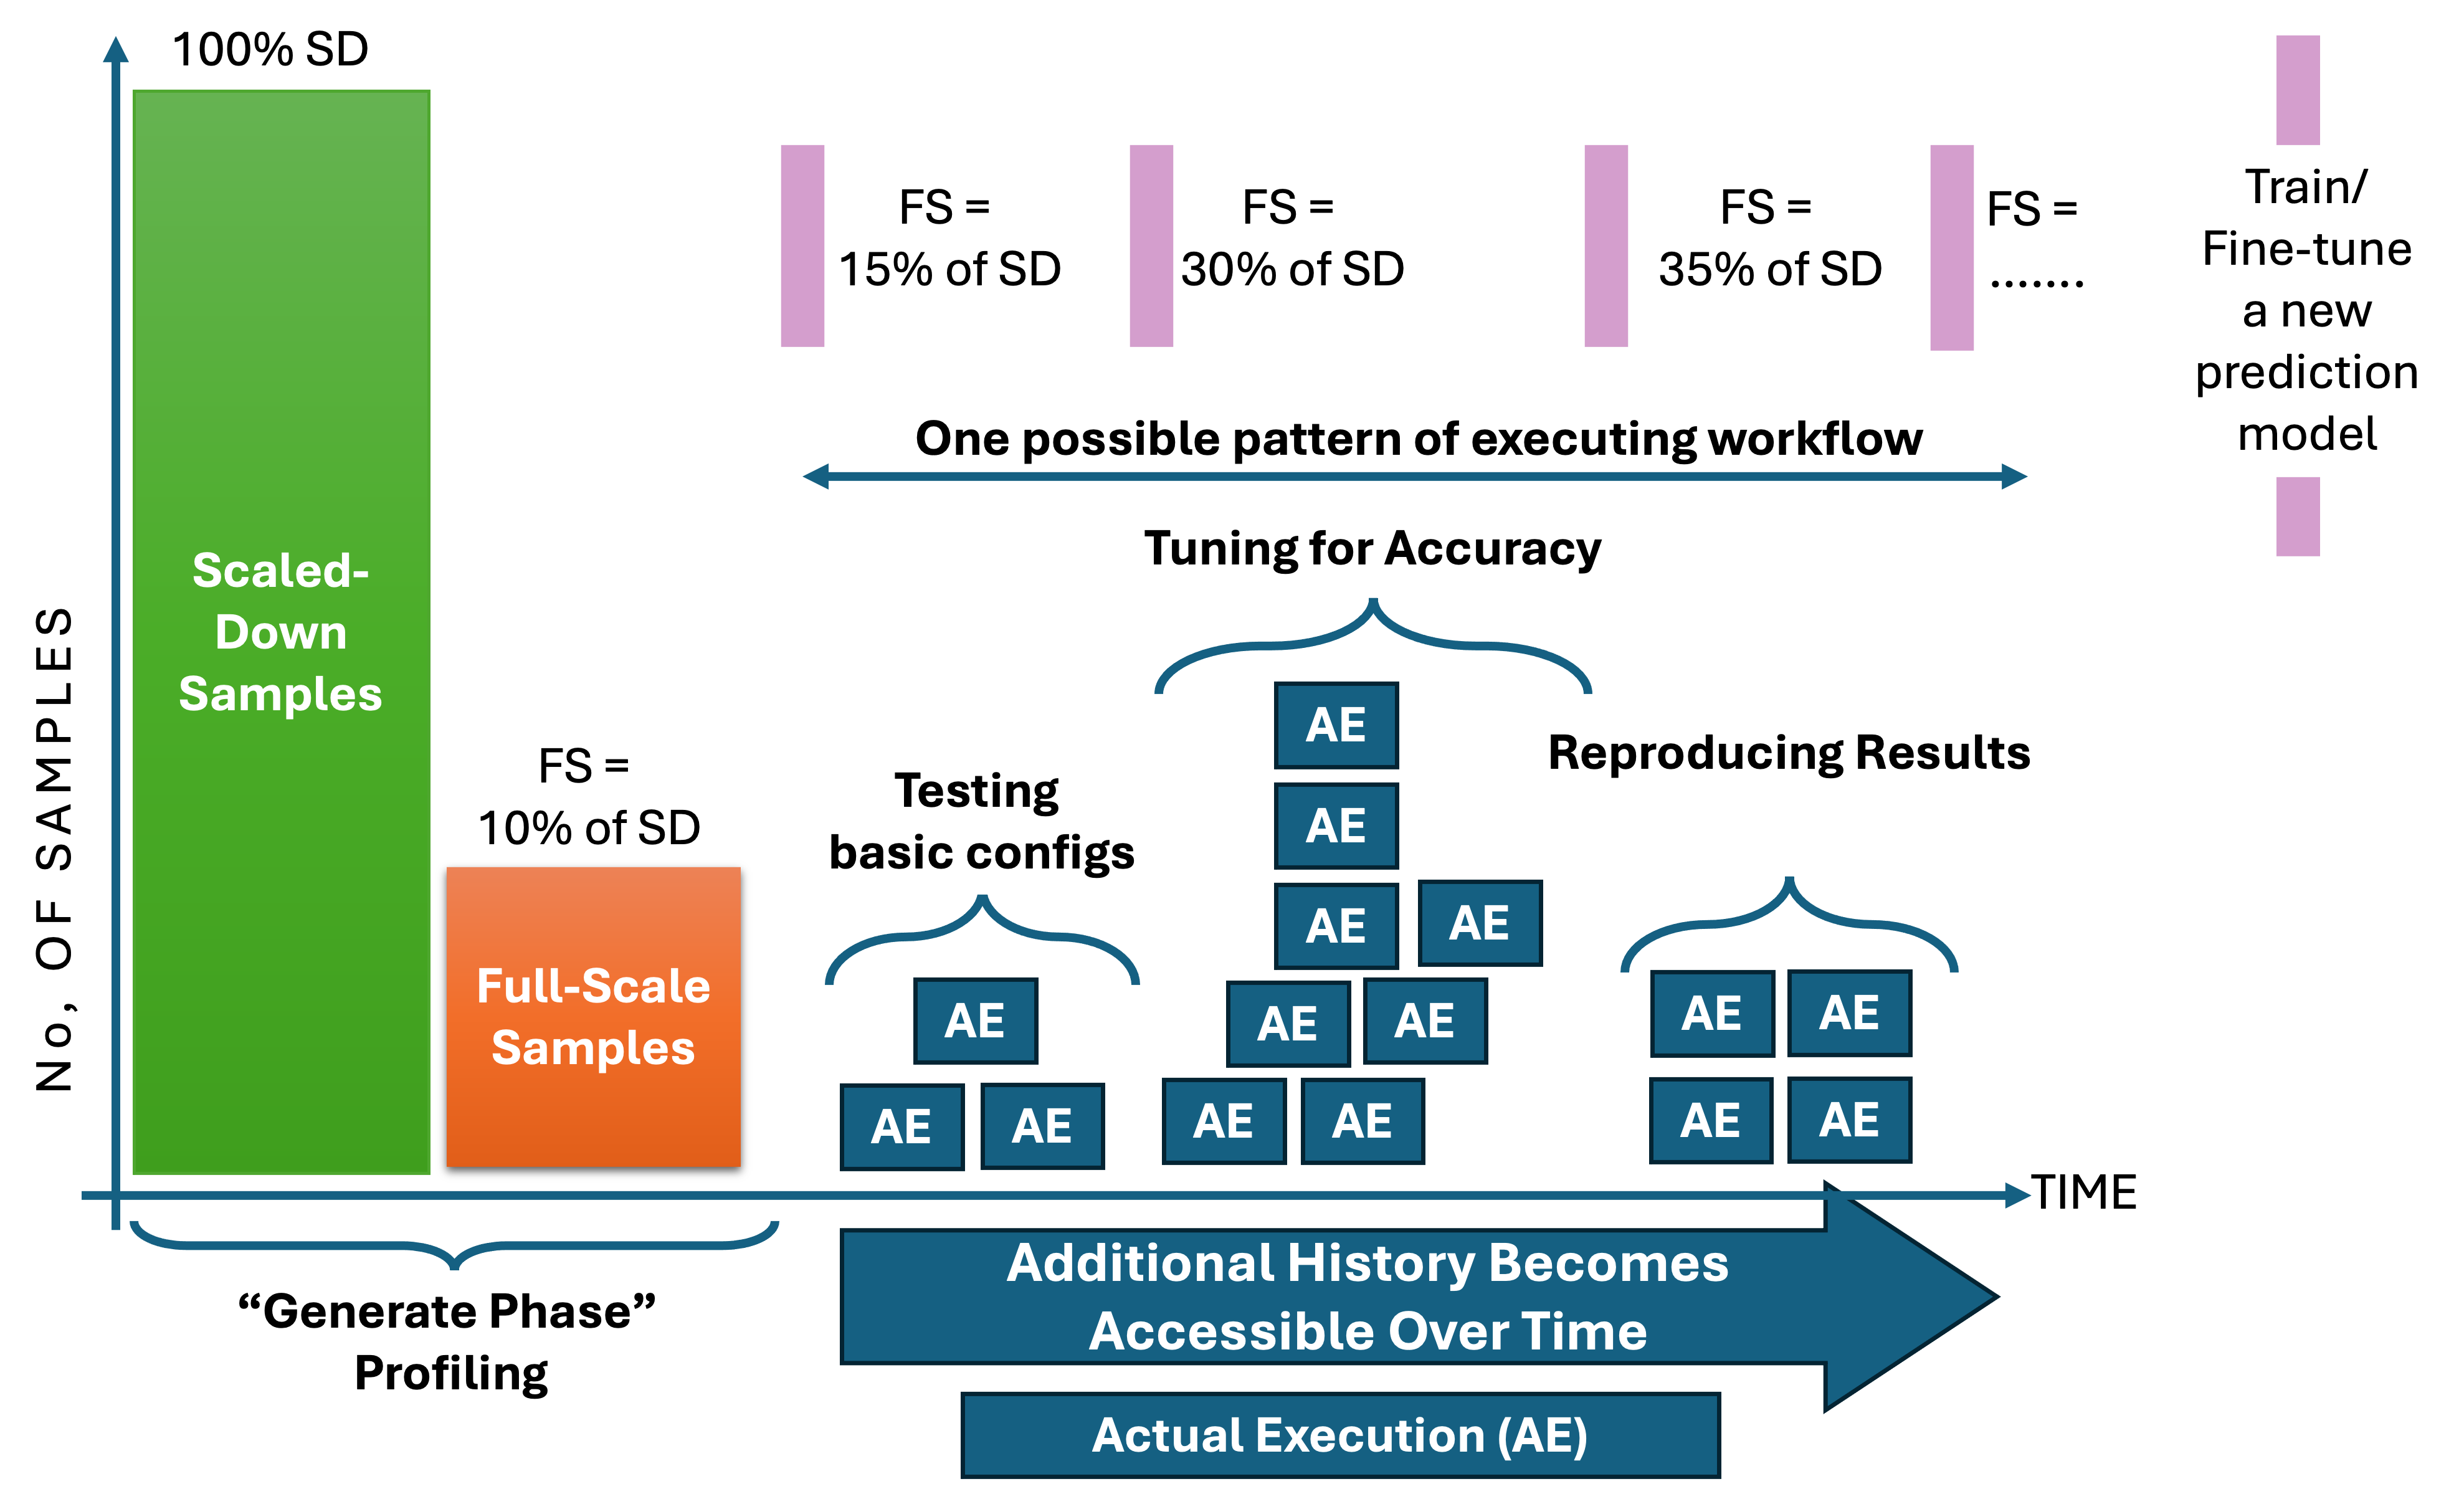
\includegraphics[width=0.9\textwidth]{Images/PatterOfDataAvial.png}
    \caption{Data availability pattern for iterative estimator fine-tuning, leveraging execution history (AE) to enhance predictions and adapt to environmental changes.}
    \label{fig:data_availability_pattern}
\end{figure}

To ensure optimal performance, our framework must support training a diverse range of regression estimators, including both off-the-shelf models and custom DNN-centric models, and dynamically select the best-performing model at any given time based on the available training data (as shown in Fig.~\ref{fig:data_availability_pattern}). The figure illustrates the data availability pattern for training and fine-tuning prediction models. As users execute jobs to test basic configurations or reproduce results, additional execution history (AE) accumulates over time. This enables iterative estimator fine-tuning, enhancing predictions, and adapting estimations to evolving environments.

We adopt a two-step approach for model selection at each retraining step:
\begin{enumerate}
    \item Train the selected models on the preprocessed training data tailored for a specific target application.
    \item Apply the model selection pipeline to identify the best-performing model among the trained models at a given instance for inference.
\end{enumerate}

\subsection{Training a Pool of Estimation Models}

Given a list of available off-the-shelf regression models (see Table~\ref{tab:Model_Chars}), all models are trained using a custom Huber loss function — an asymmetric custom loss for runtime prediction \ref{Form:Custom_Assyn_Loss}. Some models, such as Support Vector Regression (SVR), require data normalization before training, while others, like LASSO and Ridge regression, converge after applying Principal Component Analysis (PCA) and upsampling. Notably, LASSO and Ridge regression models demonstrate similar accuracy to simple linear regression, making them redundant candidates for regression models (RMs). To optimize performance, we fine-tune the hyperparameters of each model by analyzing the bias-variance tradeoff using cross-validation over the training dataset.

\subsection{Model Selection with Resource Estimation Criteria}

Among all trained models, the best-performing one is selected based on the model selection criteria (Formula~\ref{eq:Better_Model_Custom_Sel} and \ref{eq:Better_Model_Def_Criteria}). The Full-Scale (FS) Model, where both training and test samples come from Full-Scale profiles (as shown in Table~\ref{tab:ModelSelection}), is designated as the Baseline Model. The selected model is then compared against this baseline to assess its performance and robustness.

Our observations indicate that the model selection criteria consistently identify an optimal model for a given application, outperforming the baseline models. We also observe that the selected Model Type changes based on the application type, reinforcing that this pipeline is essential for making the HARP framework more application-agnostic. Additionally, it ensures that the estimators adapt dynamically to the application's characteristics and its available execution history.

% Please add the following required packages to your document preamble:
% \usepackage{multirow}
\begin{table}[]
\caption{Comparison of the Model Selected by Our Criteria Against the Baseline Model}
\label{tab:ModelSelection}
\begin{tabular}{|l|c|c|c|rrr|}
\hline
\multirow{2}{*}{\textbf{APP}} & \multicolumn{1}{l|}{\multirow{2}{*}{\textbf{Model}}} & \multirow{2}{*}{\textbf{\begin{tabular}[c]{@{}c@{}}Training \\ Data\end{tabular}}} & \multirow{2}{*}{\textbf{\begin{tabular}[c]{@{}c@{}}Model\\ Type\end{tabular}}} & \multicolumn{3}{c|}{\textbf{Metrics}} \\ \cline{5-7} 
 & \multicolumn{1}{l|}{} &  &  & \multicolumn{1}{c|}{\textbf{UPP}} & \multicolumn{1}{c|}{\textbf{MSE}} & \multicolumn{1}{l|}{MAPE} \\ \hline
\multirow{2}{*}{\textbf{\begin{tabular}[c]{@{}l@{}}Gray-\\ Scott\end{tabular}}} & \multicolumn{1}{l|}{\textbf{Baseline}} & FS & \multicolumn{1}{l|}{SVR} & \multicolumn{1}{r|}{38.30} & \multicolumn{1}{r|}{186.83} & 12.62 \\ \cline{2-7} 
 & \textbf{Selected} & \begin{tabular}[c]{@{}c@{}}SD+\\ 50\%FS\end{tabular} & DTR & \multicolumn{1}{r|}{\textbf{32.98}} & \multicolumn{1}{r|}{\textbf{120.57}} & \textbf{4.34} \\ \hline
\multirow{2}{*}{\textbf{\begin{tabular}[c]{@{}l@{}}Trimmo-\\ matic\end{tabular}}} & \textbf{Baseline} & FS & SLR & \multicolumn{1}{r|}{36.84} & \multicolumn{1}{r|}{165.82} & 3.52 \\ \cline{2-7} 
 & \textbf{Selected} & \begin{tabular}[c]{@{}c@{}}SD+\\ 50\%FS\end{tabular} & SVR & \multicolumn{1}{r|}{\textbf{7.89}} & \multicolumn{1}{r|}{\textbf{1840.32}} & \textbf{6.58} \\ \hline
\multirow{2}{*}{\textbf{\begin{tabular}[c]{@{}l@{}}Family \\ of DNNs\end{tabular}}} & \textbf{Baseline} & FS & DTR & \multicolumn{1}{r|}{35.00} & \multicolumn{1}{r|}{10.51x$10^{4}$} & 176.672 \\ \cline{2-7} 
 & \textbf{Selected} & \begin{tabular}[c]{@{}c@{}}SD+\\ 50\%FS\end{tabular} & NNR & \multicolumn{1}{r|}{\textbf{15.09}} & \multicolumn{1}{r|}{\textbf{5294.590}} & \textbf{11.800} \\ \hline
\end{tabular}
\end{table}


